\documentclass[border=4pt]{standalone}
\usepackage{tikz}
\usetikzlibrary{arrows.meta,shapes.geometric}
\begin{document}
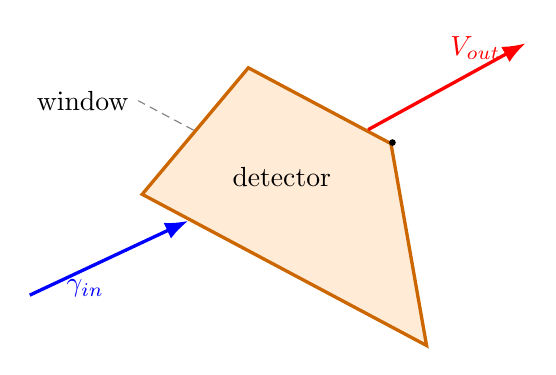
\begin{tikzpicture}[>=Latex]
  \node[
    trapezium,
    shape border uses incircle,
    shape border rotate=-28,
    trapezium left angle=78,
    trapezium right angle=52,
    minimum width=30mm,
    minimum height=15mm,
    inner sep=1mm,
    draw=orange!80!black,
    very thick,
    fill=orange!16
  ] (detector) {detector};

  \draw[-Latex,very thick,blue] (-3.2,-1.5) --
    node[pos=.35,below] {$\gamma_{in}$} (detector);
  \draw[-Latex,very thick,red] (detector) --
    node[pos=.68,above] {$V_{out}$} (3.1,1.7);
  \draw[gray,densely dashed] (detector.left side) -- ++(152:8mm)
    node[left,black] {window};
  \fill[black] (detector.top right corner) circle (1.2pt);
\end{tikzpicture}
\end{document}
